\section{Аналитический раздел}

В данном разделе представлен обзор реализаций доверенных сред исполнения и описаны их особенности. Сформулированы критерии оценки и проведено сравнение на их основе. Представлен обзор средств виртуализации в процессорных системах ARM. Представлена oформализованная постановка задачи на разработку метода программной реализации доверенной среды исполнения с помощью виртуализации процессоров архитектуры ARM.

\subsection{Анализ предметной области}

В этом разделе представлен анализ предметной области. Описаны методы обеспечения защиты информации на современных процессорах. Даны понятие и характеристика доверенной среды исполнения.

\subsubsection{Кольца привилегий}

В целях безопасности, компоненты любой системы разделены на уровни привилегий --- кольца защиты, за реализацию которых отвечает разработчик процессора. Во всех современных системах, реализована кольцевая система уровней привилегий. От внешнего кольца к внутреннему идет увеличение полномочий для инструкций кода, выполняемых на процессоре в данный момент (рисунок \ref{fig:rings}).

\begin{figure}[h]
	\centering
	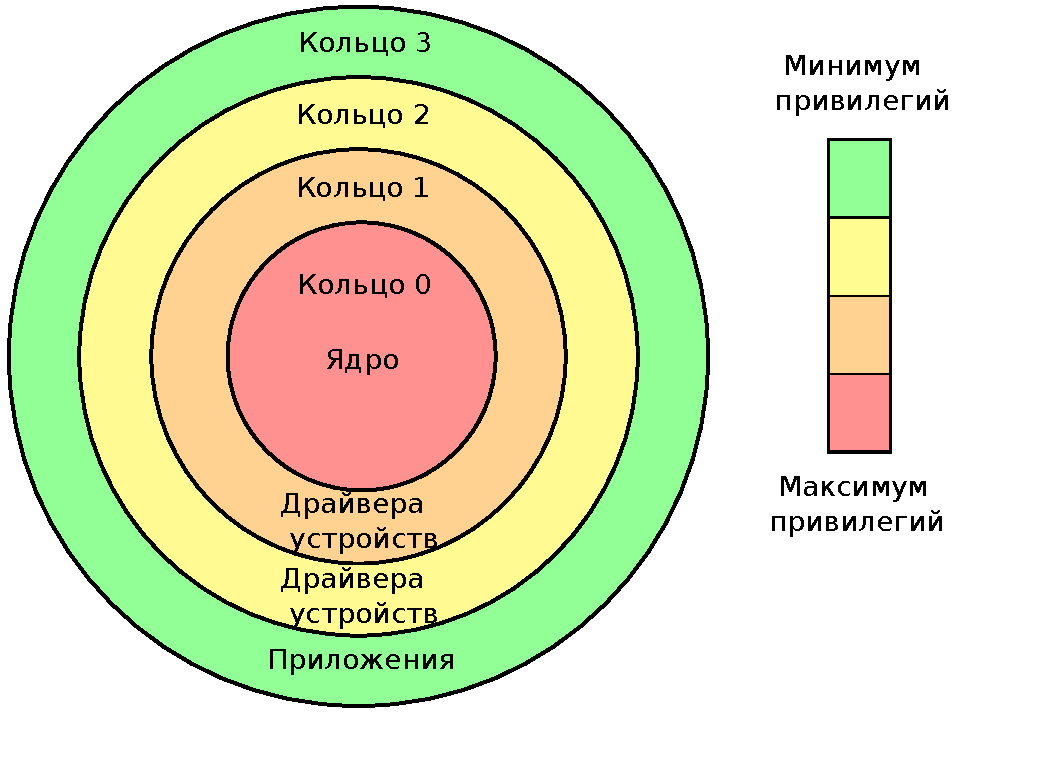
\includegraphics[width=\textwidth]{img/rings.pdf}
	\caption{Концептуальная схема представления колец защиты в современных системах}
	\label{fig:rings}
\end{figure}

Можно создавать еще более сложную систему --- формировать еще больше колец защиты, для ограничения каждого из компонентов системы. Однако, чем сложнее архитектура системы и чем больше количества кода в ней, тем проще злоумышленнику найти уязвимость и эксплуатировать ее \cite{complex-systems}.

Главной задачей злоумышленника является получение доступа к привилегиям, которые бы позволили получить доступ к необходимым ресурсам системы. Может показаться, что архитектурно верным является решение размещать конфиденциальные данные исключительно на последнем кольце защиты --- ведь получить доступ туда сложнее всего. Но у такого подхода есть свои недостатки \cite{complex-systems}. Данный подход был переосмыслен --- в настоящее используется схема, когда и код, и конфиденциальные данные хранятся на одном и том же уровне, что и пользовательские предложения, однако, доступ к ним имеет только лишь процессор. Такой метод защиты информации называется анклавом или доверенной средой исполнения.

\subsubsection{Доверенная среда исполнения}

Доверенная среда исполнения (ДСИ) --- специальная изолированная область,  которая позволяет вынести из системы часть функциональности приложений и ОС в отдельное окружение. Содержимое памяти и выполняемый код в этой среде будут недоступны из основной системы, независимо от уровня текущих привилегий. Так, например, в ДСИ выполняется код отвечающий за реализацию различных алгоритмов шифрования, обработки закрытых ключей, паролей, процедур аутентификации и работы с конфиденциальными данными. 

В случае, если система была скомпрометирована, информация хранящаяся в ДСИ не может быть определена, и доступ к ней будет ограничен лишь внешним программным интерфейсом. В отличии от других методов защиты защиты информации, таких как, например, гомоморфное шифрование, аппаратная реализация ДСИ практически не влияет на производительность системы и уменьшает время разработки программного обеспечения \cite{tee}.

С другой стороны, аппаратная реализация ДСИ имеет свои недостатки:

\begin{itemize}
	\item [---] Некоторые современные процессоры имеют лишь частичную поддержку ДСИ, либо не имеют ее вовсе.
	\item [---] Отсутствует возможности программно исправить уязвимость. Найденные уязвимости в реализации ДСИ могут быть исправлены лишь в новых ревизиях процессора, т.е. без его физической замены, злоумышленник сможет эксплуатировать уязвимость.
	\item [---] Увеличивается издержки производства на разработку таких процессоров --- их конечная стоимость возрастает.
\end{itemize}

Таким образом, в некоторых случаях, появляется необходимость в программной реализации ДСИ. Стоит отметить, что в конечном счете, программная реализация все равно использует другие аппаратные механизмы предоставляемые процессором \cite{comparsion-arm-intel}.
 
\subsection{Существующие реализации ДСИ}

\subsubsection{ARM TrustZone}\label{arm-trustzone}

ARM TrustZone --- технология аппаратного обеспечения ДСИ, разрабатываемая компанией ARM. Большинство процессоров разработанных ARM имеют поддержку TrustZone \cite{comparsion-arm-intel}. Данная технология основана на разделении режимов работы процессора на два <<мира>>: обычный мир (Normal World) и безопасный мир (Secure World). Процессор переключается в безопасный мир по запросу (с помощью специальной инструкции), при работе с конфиденциальными данными. Все остальное время, процессор работает в режиме обычного мира. Процессоры с поддержкой данной технологии имеют способность разделять память, независимо от ее типа, на ту, которая доступна только в безопасном мире, и ту, которую можно использовать в обычном мире. ARM предоставляют открытый исход программного обеспечения для поддержки данной аппаратной технологии --- ARM Trusted Firmware \cite{arm-tfa}.

\textbf{Обычный и безопасный мир.} Ключевой особенной ARM TrustZone является способность процессора переключаться между обычным и безопасным миром. Каждый из этих миров управляется собственной операционной системой, которые обеспечивают необходимую функциональность. Основное различие между этими ОС заключается в предоставляемых гарантиях безопасности. В один момент времени, процессор может находиться только в одном из двух миров, что определяется значением специального бита NS (Non-Secure), бит является частью регистра Secure Configuration Register (SCR). Этот регистр доступен для периферии только для чтения, изменять его значение может лишь сам процессор. Когда процессор находится в обычном режиме исполнения кода, значение бита NS равно 1, и наоборот, когда процессор находится в безопасном мире, значение бита NS равно 0.

За связь между обычным и безопасным миром отвечает специальный механизм --- Secure Monitor. Он соединяет оба мира и является единственной точкой входа в безопасный мир. Для того, чтобы из обычного мира перейти в безопасный, существует специальная инструкция процессоров ARM --- Secure\\Monitor Call (SMC). При вызове данной инструкции процессор передает управление Secure Monitor. Тот в свою очередь готовит систему к переходу из одного мира в другой и передает управление соответствующей ОС. Инструкция SMC используется как для перехода из нормального мира в безопасный, так и для перехода из безопасного в нормальный. Некоторые прерывания или исключения могут быть настроены так, чтобы они так же проходили через Secure Monitor и были обработаны в безопасном мире. ARM предоставляет спецификацию Secure Monitor Call Calling Convention (SMCCC) \cite{smccc}, которая является стандартом при реализации вызовов SMC. 

На рисунке \ref{fig:trustzone-conceptual} представлена концептуальная схема взаимодействия двух миров.

\begin{figure}[h]
	\centering
	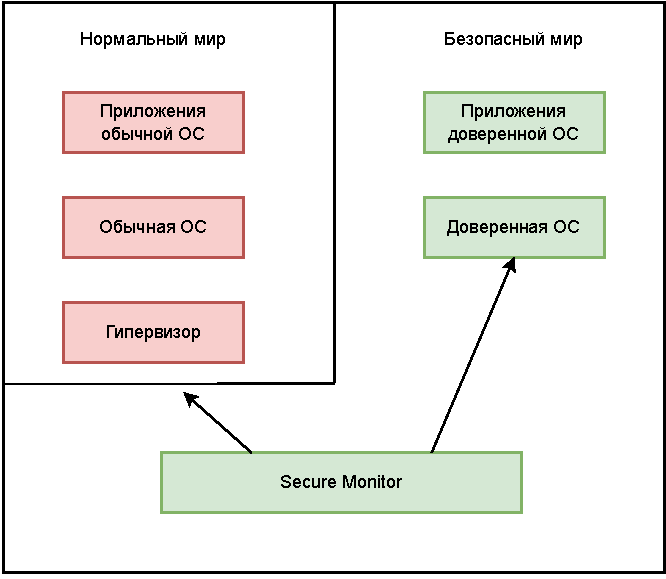
\includegraphics[width=\textwidth]{img/arm-conceptual.pdf}
	\caption{Концептуальная схема взаимодействия двух миров для процессоров ARM Cotrex-A}
	\label{fig:trustzone-conceptual}
\end{figure}

Доверенная операционная система, так же как и обычная, может запускать приложения. Они, как и в обычном мире, обращаются к доверенной ОС при необходимости получения каких-либо ресурсов или обработки прерываний и исключений. Таким образом, Secure Monitor передает управление одному из доверенных приложений, и уже те, в свою очередь, обращаются к доверенной ОС.

ARM предоставляют открытый исходной код эталонной доверенной операционной системы, которая называется OP-TEE \cite{optee}. Global Platform предоставляет спецификацию для реализации API взаимодействия доверенных приложений \cite{teec-spec} с доверенной ОС \cite{tee-spec}.

Физически миры разделены таким образом, что часть регистров доступны только в безопасном мире. Периферия, например память, может быть настроена так, что она может быть доступна лишь в определенном мире. Технология TrustZone в нормальном режиме работы процессора не позволяет программному обеспечению получить доступ к аппаратным средствам, которые могут быть доступны лишь только в безопасном мире. 

При сборке компонентов системы, производитель устройства должен позаботиться о конфигурации периферии для работы с TrustZone:

\begin{itemize}
	\item [---] если предполагается, что периферия может получать доступ к безопасному режиму исполнения, процессор и внешнее устройство должны быть соединены (помимо различных шин) линией NS. Получение сигнал NS=0 от процессора к периферии означает, что команда является доверенной (например операция чтения или записи).
	\item [---] В обратном случае, линия NS может быть опущена. Предполагается, что такая периферия не имеет никаких привилегий, т.е. NS=1 всегда.
\end{itemize}

На рисунке \ref{fig:ns-bit} представлена схема взаимодействия процессора и периферии для поддержки TrustZone. Периферийные устройства №1 и №3 соединены линией NS, а устройство №2 нет.

\begin{figure}[h]
	\centering
	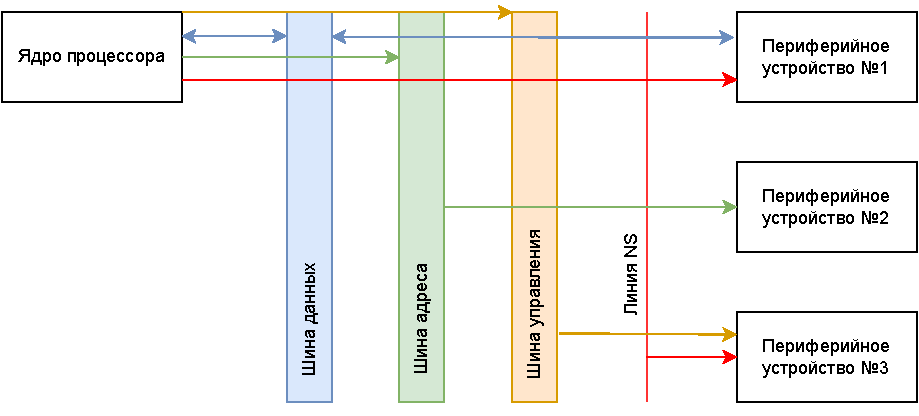
\includegraphics[width=\textwidth]{img/arm-ns.pdf}
	\caption{Пример взаимодействия процессора и периферии для поддержки TrustZone}
	\label{fig:ns-bit}
\end{figure}

Стоит отметить, что чаще всего не вся периферия соединена сигналом NS с процессором. Например, тот факт, что производитель устройства не соединил сигналом NS камеру и ядра процессора, полностью исключает возможность предоставления пользователю доступа к устройству с помощью технологии распознавания лица.

\textbf{Режимы работы процессора.} Современная архитектура ARM поддерживается три режима работы процессора: 

\begin{itemize}
	\item [---] \texttt{EL0} --- непривилегированный режим работы, предназначенный для исполнения обычных программ;
	\item [---] \texttt{EL1} --- привилегированный режим работы --- исполняется код ОС, обработчиков прерываний и исключений;
	\item [---] \texttt{EL2} --- режим работы гипервизора.
\end{itemize}

Для того, чтобы программа исполняемая на уровне EL0 могла перейти в EL1 (например, обратиться к ресурсам доступным только ОС), в архитектуре ARM существует команда Supervisor Call (SVC). Аналогично, Hypervisor Call (HVC) предназначена для перехода из режима EL1 в EL2.

Каждый из этих уровней могут исполняться в нормальных (Non-Secure) так и безопасных (Secure) режимах (рисунок \ref{fig:arm-levels}).

\begin{figure}[h]
	\centering
	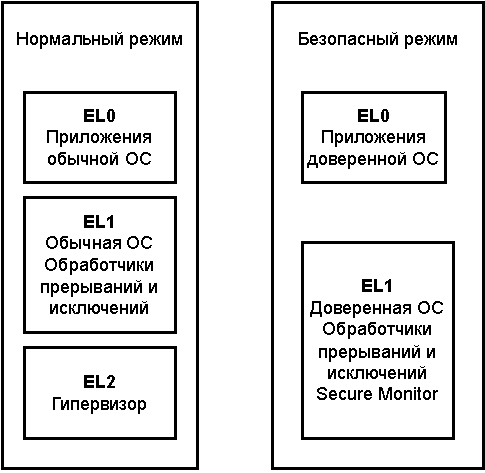
\includegraphics[width=\textwidth]{img/arm-levels.pdf}
	\caption{Режимы работы процессоров архитектуры ARM}
	\label{fig:arm-levels}
\end{figure}

\begin{itemize}
	\item [---] Обычные приложения исполняются на уровне Non-Secure EL0, а приложения доверенной ОС на Secure EL0.
	\item [---] Обычная ОС выполняется на уровне Non-Secure EL1. Все прерывания и исключения произошедшие в нормальном мире так же обрабатываются на этом уровне; доверенная ОС и прерывания произошедшие в безопасном мире исполняются на уровне Secure EL1.
	\item [---] Secure Monitor всегда исполняется на уровне Secure EL1.
	\item [---] Гипервизор исполняется в режиме Non-Secure EL2.
\end{itemize}

Бит NS, который был описан в предыдущей главе, определяет то, в каком режиме сейчас исполняется код: обычном (NS=1) или безопасном (NS=1).

Благодаря дублированию нормального и безопасного режима архитектура ARM позволяет запустить сразу две ОС: обычную и доверенную.

\textbf{Разделение памяти.} В целях безопасности в ARM TrustZone память разделяется на защищенную и незащищенную область. Благодаря контроллеру адресного пространства (TZASC --- TrustZone Address Space Controller) незащищенная область память может использоваться только из обычного мира, а защищенная из безопасного. Кэш память так же разделяется на защищенную и незащищенную. Необходимо отметить, что данный контролер не является обязательным в архитектуры ARM TrustZone, поэтому разработчики могут принять решение отказаться от них в пользу более компактных и менее энергоемких устройств.

\textbf{Проверка целостности.} Проверка целостности ДСИ является важным механизмом, который не позволит злоумышленнику изменить исходный код доверенной ОС или доверенных приложений. В ARM TrustZone данный механизм реализован на аппаратном уровне как для ОС, так и для приложений: каждый раз, при загрузке доверенной ОС в память, с помощью цифровой подписи проверяются ее целостность. Аналогичная схема используется и при загрузке доверенных приложений. Запустить ОС может только подписанные приложения, подпись формируется разработчиками, на стадии компиляции в исполняемый файл.

На данный момент, доверенная среда исполнения от компании ARM не поддерживает процедуру удаленной проверенной проверки (например, с помощью сервера). Существуют лишь программные решения этой проблемы от сторонних разработчиков \cite{comparsion-arm-intel}.


\subsubsection{Intel SGX}

Intel Software Guard Extension (SGX) --- реализация ДСИ от компании Intel, включена в большинство современных процессоров Intel Core. Конфиденциальность и целостность в этой технологии достигается с помощью использования анклава --- специальной, зашифрованнаой области кода и данных. Это достигается с помощью различных компонентов и протоколов, одним из которых является специальная область памяти, называемая Processor Reserved Memory (PRM), обеспечивающая безопасное хранилище, к которому не может обращаться никто, кроме самого процессора. Для выполнения кода, после череды его проверок, он загружается извне в PRM. Процессор с помощью специальных инструкций переходит в режим анклава (enclave mode) и выполняет загруженный код. В технологии Intel SGX именно анклав является доверенной средой исполнения.

\textbf{Processor Reserved Memory.} Processor Reserved Memory (PRM) --- защищенная часть оперативной памяти, к которой не имеет доступ код, который исполняет в режиме non-enclave. Это реализуется аппаратно, с помощью специальных контроллеров доступа к памяти. 

Данный участок памяти подразделяется на дополнительные разделы.

\begin{itemize}
	\item [---] Encalve Page Cache (EPC) --- разделенная страницы размером 4Кб область памяти, которые хранят код конкретного анклава, к которому относятся; это позволяет использовать в системе несколько анклавов одновременно. EPC управляется программным путем с помощью ОС. Доступ к нему может быть получен только программным обеспечением входящим в данный анклав.
	\item [---] Enclave Page Cache Map (EPCM) --- массив с одной записью для каждой страницы, хранимой в EPC; запись содержит в себе метаданные этой страницы: владелец, виртуальный адрес и т. д.
	\item [---] SGX Enclave Control Structure (SECS) --- содержит в себе метаданные соответствующего анклава; хранится в специальной страничной части EPC. Страница, ассоциированная с SECS не отображается в память напрямую и доступна только для реализации SGX --- это сделано в целях дополнительной безопасности.
\end{itemize}

Схема представления памяти с использованием Intel SGX представлена на рисунке \ref{fig:intel-prm}.

\begin{figure}[h!]
	\centering
	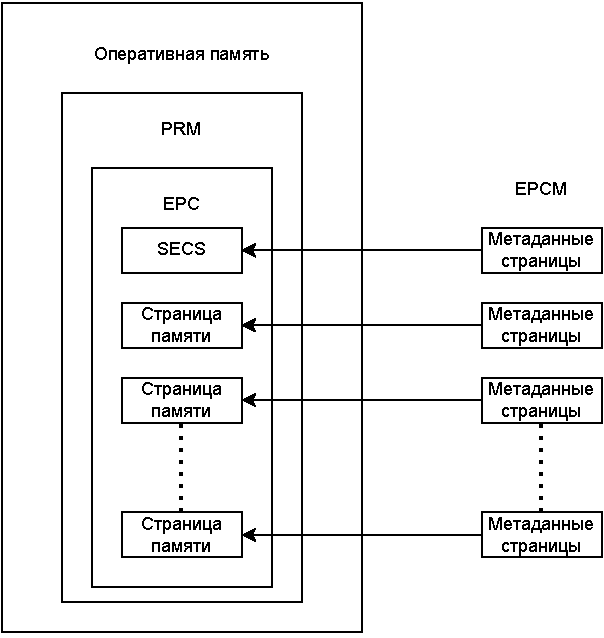
\includegraphics[width=\textwidth]{img/intel-prm.pdf}
	\caption{Схема представления памяти Intel SGX}
	\label{fig:intel-prm}
\end{figure}

Анклав получает доступ к EPC, выделяя часть своей виртуальной памяти под линейный диапазон адресов анклава (Enclave Linear Address Range,\\ELRANGE), который содержит адреса сопоставленные с EPC. Другие адреса виртуальной памяти отображаются на память расположенную за пределами EPC. Процессор проверяет что в результате трансляции физического адреса страницы, находящейся в EPC, виртуальный адрес совпадает с адресом хранящимся в EPCM --- это позволяет предотвратить атаки на трансляцию адресов.

Каждая страница обладают индивидуальными правами доступа, которые устанавливаются при выделении соответствующей страницы и определяются автором анклава, что так же является дополнительной мерой безопасности. Страницы разделены на те, которым разрешено чтение, запись и выполнение кода анклава. Эта информация так же находится в метаданных страницы, хранящихся EPCM.

State Save Area (SSA) --- еще один компонент Intel SGX, отвечающий за сохранение текущего состава анклава. Это специальная область памяти, которая используется для хранения контекста выполнения кода анклава. Эта область памяти необходима, например, когда в системе произошло прерывание --- процессору необходимо перейти в нормальный режим исполнения для его обработки. После этого, процессор может загрузить состояние анклава из SSA и возобновить выполнение кода.

Еще одной особенностью с точки зрения безопасности и производительности, является возможность вытеснения страниц из PRM в обычную (не-PRM) память. Большинство современных компьютеров поддерживают избыточное использование оперативной памяти, выгружая некоторые страницы во вторичные устройства. Технология Intel SGX поддерживает это, добавляя меры, которые гарантирую целостность и конфиденциальность вытесняемых страниц: вытесняемая страницы шифруется с помощью симметричного шифрования, а ключ хранится в специально отведенных для этого страницах EPC.

\textbf{Жизненный цикл анклава.} Для управления анклавами Intel предоставляет набор специальных инструкций:

\begin{itemize}
	\item [---] \texttt{ECREATE} --- создает новый анклав и сохраняет его метаданные в SECS.
	\item [---] \texttt{EADD} --- используется для добавления новых страниц в анклав; ОС загружает новый страницы в EPC, заполняя необходимые метаданные. Вызывать эту инструкцию можно только после создания анклава, попытка добавить страницы после этого этапа приведет к ошибке.
	\item [---] С помощью инструкции \texttt{EINIT} и специального токена от Launch Enclave, процессор начинает выполнять код анклава. Launch Encalve --- специальный анклав, проходящий все те же стадии инициализации, что и другие. Его основная цель является выдача токена другим анклава на основе списка одобренных анклавов.
	\item [---] Приложения могут выполнить команду \texttt{EENTER} для входа в режиме анклава и выполнения там своего кода, по окончанию выйти оттуда используя команду \texttt{EEXIT}. В виртуальном адресном пространстве этих приложений должны иметься соответствующие страницы EPC.
	\item [---] Команда \texttt{AEX} используется при возникновении прерывания или исключения, после ее выполнения процессор переходит в обычный режим исполнения, сохраняя контекст в SSA.
	\item [---] \texttt{ERESUME} --- возобновить выполнение анклава с контекстом, сохраненным в SSA. Стоит отметить, что анклав может иметь более одного SSA в случаях, если при выполнении одного и того же блока происходит несколько прерываний.
\end{itemize}

После выполнения кода, в метаданных страниц, ассоциированных с этим анклавом, выставляется пометка, что они невалидны. После этого очищается TLB кэш. Это позволяет защитить Intel SGX от атак на память. На рисунке \ref{fig:enclave-life} представлена схема жизненного цикла анклава с использованием команд, описанных выше.

\begin{figure}[h]
	\centering
	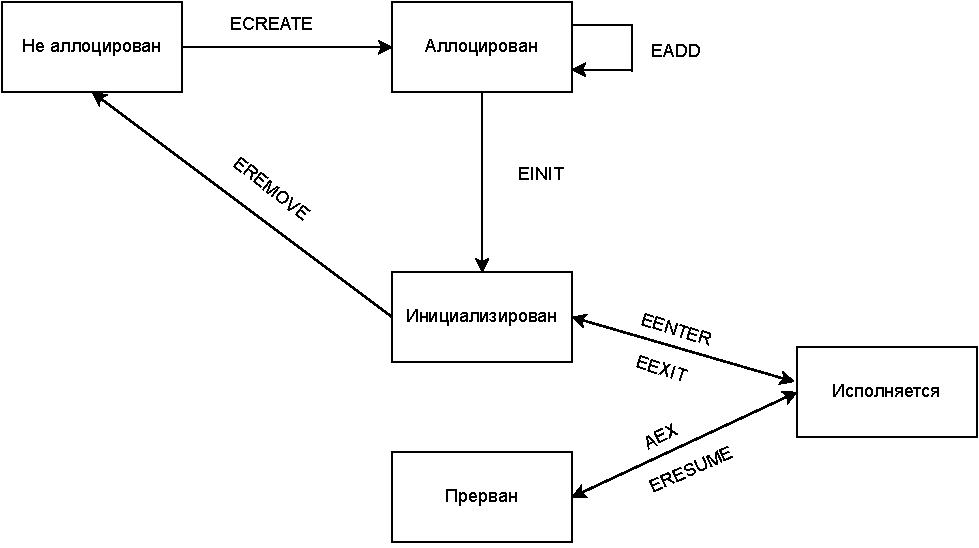
\includegraphics[width=\textwidth]{img/enclave-life-cycle.pdf}
	\caption{Жизненный цикл анклава}
	\label{fig:enclave-life}
\end{figure}

\textbf{Проверка целостности.} В Intel SGX реализована поддержка механизма локальной и удаленной  проверки целостности. 

Локальная проверка используется для установления канала связи, который гарантирует конфиденциальность, двумя анклавами на одном устройстве. Для обмена симметричными ключом используется протокол  Диффи-Хеллмана \cite{dh-ke}. Локальная проверка начинается с того, что один из анклавов отправляет значение MRENCLAVE (индивидуальный идентификатор анклава) другому анклаву, который находится на том же устройстве. Отправитель называется верификатором, а получающий анклав утверждающим. Отправитель использует полученное от верификатора значение MRENCLAVE для создания отчета (claimer), который он отправляет обратно верификатору. Отчет может быть проверен с помощью специально ключа REPORT KEY, который хранится на устройстве и доступен всем анклавам. Он так же содержит данные обмена ключами Диффи-Хеллмана, который в дальнейшем будут использованы для создания защищенного канала связи. После проверки отчета, верификатор создает и отправляет отчет для утверждающего анклава. Затем обе стороны могут создать защинный канал используя данные Диффи-Хеллмана, содержащиеся в обоих отчетах. На рисунке \ref{fig:enclave-local-attestation} представлена схема локальной проверки целостности в Intel SGX.

\begin{figure}[h]
	\centering
	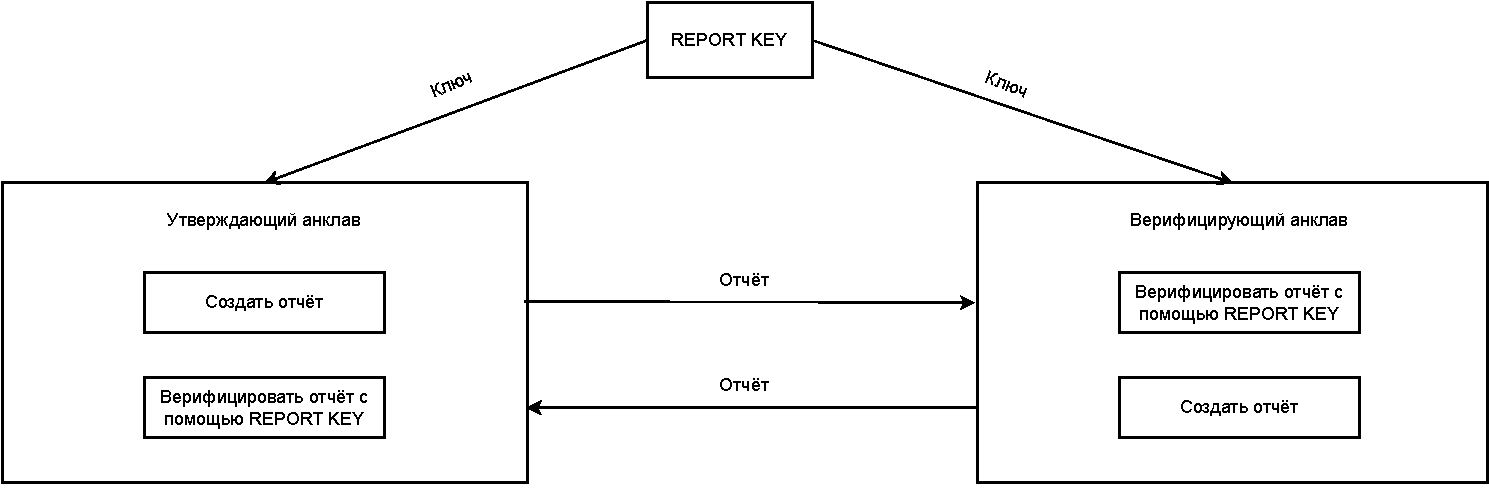
\includegraphics[width=\textwidth]{img/enclave-local-attestation.pdf}
	\caption{Схема локальной проверки целостности в Intel SGX}
	\label{fig:enclave-local-attestation}
\end{figure}

Удаленная проверка целостности реализовывается с помощью удаленной службы Intel Attestation Service \cite{intel-attestation-service}. В процессе проверки, используется подсчет хэш-суммы анклава с помощью хэш-фукнции SHA-2 \cite{sha2}, специального анклава находящегося в однократно записываемой памяти и ключей, которые были расположены в устройстве на стадии его производства. С помощью ключей и хэш-суммы, анклав расположенный в однократно записываемой памяти формирует специальный отчет, отправляемый в службу Intel Attestation Service, и та, в свою очередь, на основе этого отчета проверяет целостность анклава.

\subsubsection{Keystone}

Keystone --- реализация доверенной среды с открытым исходным кодом для процессоров на базе архитектуры RISC-V. В отличии от Intel SGX и ARM TrustZone, эта технология является полностью программным решением с открытым исходным кодом, построенным на использовании аппаратных особенностей архитектуры RISC-V. Keystone предоставляет спецификацию для разработчиков устройств, выполнение которой гарантирует поддержку этого механизма \cite{riscv-keystone}.

\textbf{Компоненты системы.} Keystone состоит из нескольких компонентов, каждый из которых выполняются на разном уровне привилегий \cite{keystone-overview}.

Всего есть три уровня привилегий:

\begin{itemize}
	\item [---] \texttt{U-mode} (user) --- режим исполнения пользовательских процессов;
	\item [---] \texttt{S-mode} (supervisor) --- режим выполнения кода ядра;
	\item [---] \texttt{M-mode} (machine) --- режим, в котором осуществляется доступ к периферии устройства.
\end{itemize}

Ниже будут описаны компоненты, с помощью которых строится доверенная среда исполнения Keystone.

Trusted Hardware --- совместимые со спецификацией Keystone ядра архитектуры RISC-V и ключи (открытый и закрытый), используемые для подписи анклава. Аппаратное обеспечение также может содержать дополнительные функции, например разделение кэша, шифрование памяти, криптографический защищенный источник случайных чисел.

Security Monitor (SM) --- выполняется в режиме M. Предоставляет интерфейс для управления жизненным циклом анклава, а так же для использования специфических возможностей платформы. SM обеспечивает выполнение гарантий безопасности Keystone, поскольку он отвечает за изоляцию анклавов и обычной (недоверенной) ОС. 

Анклавы представляет собой среду, изолированную от операционной системы и других анклавов. Каждому анклаву выделяется отдельная область физической памяти, получить доступ к которой может только он сам и Security Monitor. Каждый анклав состоит из анклавного приложения, выполняемого на уровне пользователя (режим  U) и Runtime (режим S).

Приложения анклава (EAPP) --- приложение пользовательского уровня, которого выполняется в анклаве. Можно создавать собственное приложение с нуля или просто запустить существующий исполняемый файл.

Runtime --- программное обеспечение выполняющиеся в режиме S, реализующие такие следующий возможности: системные вызовы, управление виртуальной памятью, обработка прерываний и так далее.

На рисунке \ref{fig:riscv-enclave-arch} представлена концептуальная схема компонентов системы ДСИ Keystone.

\begin{figure}[h]
	\centering
	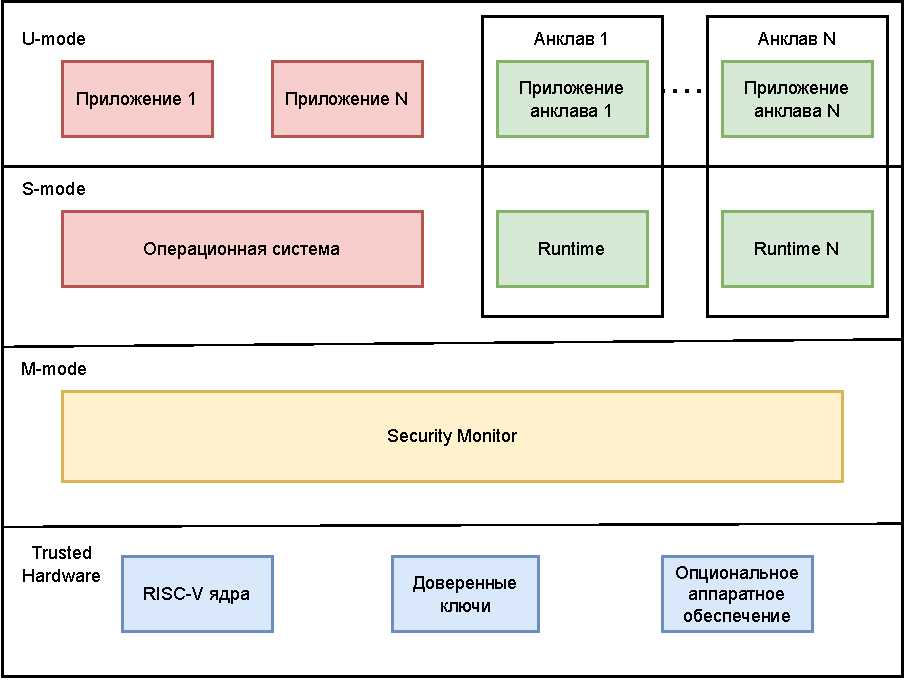
\includegraphics[width=\textwidth]{img/riscv-enclave-arch.pdf}
	\caption{Компоненты системы доверенной среды исполнения Keystone}
	\label{fig:riscv-enclave-arch}
\end{figure}

\textbf{Жизненный цикл анклава.} Анклав Keystone может находится в трех состояниях \cite{keystone-overview}.

\begin{enumerate}[label*=\arabic*.]
	\item Создание. Анклав загружается на непрерывный диапазон физической памяти, которая называется приватной памятью анклава. Недоверенный код (например, операционная система) выделяет эту память и инициализирует таблицу страниц анклава, загружает код компонента Runtime и приложение анклава. Для создания анклава вызывается Secure Monitor, которые изолирует и защищает приватную память с помощью механизма защиты физической памяти, что позволяет защитить память анклава от изменений и чтений для любого ядра процессора. После выполнения этих действий, SM помечает анклав  готовым для выполнения.
	\item Выполнение. Недоверенный код запрашивает у SM разрешение на исполнение кода анклава на одном из ядер процессора; SM выдает разрешение на выполнение и ядро начинает выполнять его код. Процесс выполнения может быть прерван (например для обработки прерывания), и, в таком случае, ядро перестанет выполнять код анклава и уберет разрешение на выполнение его кода.
	\item Разрушение. Недоверенный код может уничтожить анклав в любое время. При его уничтожении, SM освобождает выделенную память для анклава, снимает с нее защиту и передает ее в распоряжение операционной системы, предварительно заполнив нулями ее содержимое.
\end{enumerate}

На рисунке \ref{fig:riscv-enclave-lifecycle} представлена схема жизненного цикла анклава Keystone.

\begin{figure}[h]
	\centering
	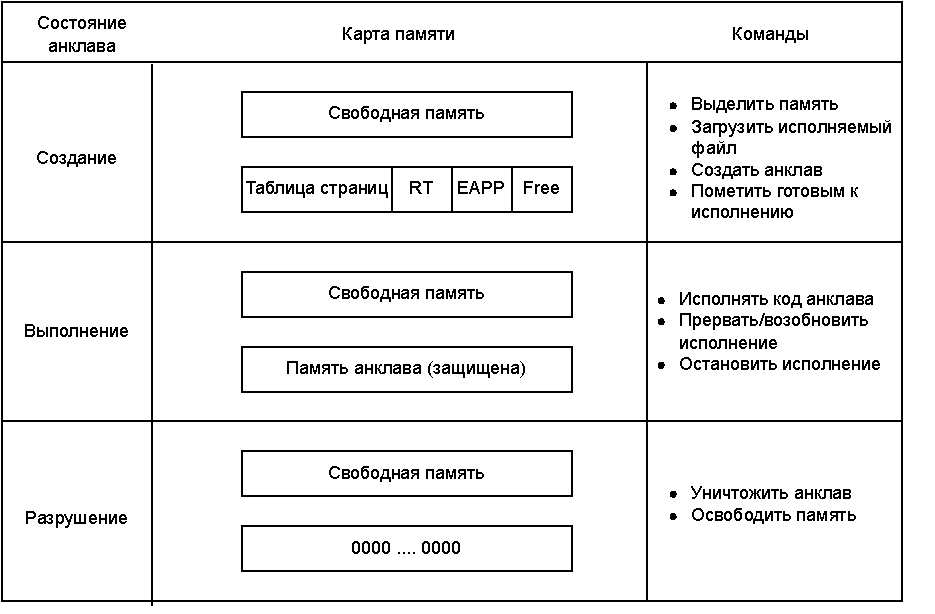
\includegraphics[width=\textwidth]{img/riscv-enclave-lifecycle.pdf}
	\caption{Жизненный цикл анклава}
	\label{fig:riscv-enclave-lifecycle}
\end{figure}

При создании анклава, участок его памяти состоит из таблицы страницы, компонента Runtime, приложения и свободного участка памяти. При его уничтожении, она предварительно заполняется нулями.

\textbf{Проверка целостности.} Архитектура ДСИ Keystone предполагает использование как локальной, так и удаленной проверки целостности анклава.

Для того чтобы локально проверить целостность анклава, при его создании вычисляется хэш-сумма (на основе кода и данных). Далее, анклав генерирует ключ шифрования, который будет использоваться для аутентификации анклава и защиты его кода и данных. Ключ подписывается с помощью доверенного ключа (см. рисунок \ref{fig:riscv-enclave-arch}), для удостоверения его подлинность. Ключ анклава и информация о нем, включая его хэш-сумму и сертификат, передаются клиенту (например, хост-системе), который будет проверять анклав. Клиент проверяет аутентичность хэш-суммы анклава и его ключа, используя доверенный открытый ключ. Если анклав и его ключ прошли проверку, клиент может быть уверен в его подлинности и целостности.

\subsection{Виды угроз безопасности}
\label{sec:security}

Существует множество различных видов атак, которые могут быть направлены на компрометацию доверенных сред исполнения. В конечном итоге, они приводят к опасности для целостности кода и данных, хранящихся внутри ДСИ. В этом разделе будут описаны наиболее распространенные виды атак.

\subsubsection{Физические атаки}

Физические атаки обычно связаны с использованием аппаратных средств или их эксплуатацией \cite{attack-on-chip}. Ниже будут приведены наиболее распространенные типы физически атак на устройство.

Самая простая атака типа отказ в обслуживании, заключается в отключении питания компьютера или другого электрического оборудования и предотвращении его использования. Более продвинутые методы включают в себя подключение USB накопителей и загрузка устройства таким образом, чтобы получить доступ к периферии и кражу ключей шифрования.

Прослушивание шины \cite{attack-on-chip} --- контролируя шину на материнской плате компьютера, злоумышленники могут подслушивать трафик, и возможно, даже его модифицировать, добавляя, удаляя или воспроизводя старые новые.

Другой подход к физическим атакам заключается в мониторинге энергопотребления процессора и вывод о типе вычислений, выполняемых в данный момент. Такой тип атаки называется атакой анализа энергопотребления (англ. Power Analysis Attack \cite{power-analysis-attack}). Он может быть использован против ДСИ, поскольку легко выявить паттерн их вычислений.

Атаки на чип \cite{attack-on-chip} --- еще один вид физической атаки. В этих атаках используются ионно-лучевые инструменты для атак на микросхемы. Суть этих атак заключается в изменении поведения аппаратных средств микросхем таким образом, чтобы обходить механизмы защиты. Например, с помощью такого вид атак, можно добиться чтобы процессор пропускал некоторые инструкции ПО.

\subsubsection{Атаки на привилегированное ПО}

Атаки на привилегированное ПО является одной из главных проблем всех ДСИ. Атаки этого типа предполагают, что они могут происходить со всех уровней привилегий. Такие типы атак включают в себя получение доступа к режиму управления всей системой, т.е. получение доступа к наиболее привилегированному режиму работы ПО в системе. Раньше, доступ к такому режиму был возможен только с помощью аппаратных средств, но с недавнего времени и с помощью программных \cite{comparsion-arm-intel}, что позволяет атакам этого типа эксплуатировать это.

\subsubsection{Программные атаки на периферию}

Другой формой атаки является использование периферийных устройств или их интерфейсов для получения доступа к памяти или для реализации других атак. Такие атаки не требуют аппаратного обеспечения или физического воздействия на устройство. 

Примером такой атаки является атака rowhammer \cite{rowhammer}. Суть атаки заключается в многократной записи в одну и ту же ячейку памяти, что приводит к изменению значения соседних ячеек, т.е. эксплуатация аппаратной особенности. Многократно изменяя значения определенных адресов памяти, злоумышленник может изменить структуры данных, отвечающие за безопасность систем, таким образом, чтобы получить привилегии суперпользователя.

Другой разновидность подобных атак является злоупотребление определенными функциями ПО в злонамеренных целях. Например, использование функций мониторинга производительности и температуры процессоров для получения информации об его активности и текущих вычислений.

\subsubsection{Трансляция адресов}

Другой серьезной проблемой для ДСИ являются атаки на трансляцию адресов, особенно для Intel SGX и Keystone, в которых процесс трансляции адресов управляется недоверенным системным ПО, в отличии от ARM TrustZone (управляется доверенной ОС).

Одним из типов данного вида атаки заставляет ОС перестроить память таким образом, чтобы выполнить нежелательные инструкции. Например, ОС может менять местами содержимое двух ячеек памяти, содержащих разные наборы инструкций, причем один набор из наборов является вредоносным. В результате, атакованное приложение выполнит вредоносные инструкции, что может привести к раскрытию ключей шифрования, пользовательских данных и другой конфиденциальной информации.

Еще одни слабым местом является вытеснение памяти из защищенной в незащищенную. Когда память перераспределяется в защищенную, ОС может без каких-либо проверок загрузить ее и передать управление приложению, которое начнет исполнять инструкции. ДСИ должны быть защищены от таких атак, отслеживая корректный виртуальный адрес для каждой физической ячейки и связывать каждый вытесняемый фрагмент памяти к правильному виртуальному адресу. Однако, даже этого может оказаться недостаточным, потому что злоумышленник может воздействовать на TLB-кэш, хранящий результаты транслирования адресов \cite{attack-on-chip}.

\subsection{Сравнение реализаций ДСИ}

\subsubsection{Критерии сравнения}

Для сравнения раннее описанных реализаций ДСИ были выделены следующие критерии:

\begin{itemize}
	\item [---] К1 --- безопасность;
	\item [---] K2 --- производительность (место);
	\item [---] К3 --- полнота и надежность механизмов проверки целостности ДСИ;
	\item [---] К4 --- является проприетарным решением;
	\item [---] К5 --- программное или аппаратное решение.
\end{itemize}

\subsubsection{Сравнение безопасности}

В таблице \ref{table:security-features} приведено сравнение защиты ДСИ от видов атак, описанных в разделе \ref{sec:security}.

\begin{table}[!htb]
	\begin{center}
		\caption{Результаты сравнения безопасности ДСИ}
		\label{table:security-features}
		\begin{tabular}{|c|c|c|c|}
			\hline
			& \bfseries TrustZone & \bfseries Intel SGX & \bfseries Keystone \\
			\hline
			\bfseries Физические атаки & - & - & - \\ \hline
			\bfseries Атаки на привилегированное ПО & + & + & + \\ \hline
			\bfseries Программные атаки на периферию & + & + & + \\ \hline	
			\bfseries Трансляция адресов & + & + & + \\ \hline	
		\end{tabular}
	\end{center}
\end{table}

\begin{itemize}
	\item [---] Ни одна из реализаций ДСИ, рассмотренных в данной работе, никак не защищена от физических атак.
	\item [---] Intel SGX и Keystone защищены от атак на привилегированное ПО, потому что оно не является доверенным и не может получить доступ к памяти анклава. Разделение на доверенную и недоверенную ОС в ARM TrustZone так же позволяет сделать вывод о том, что данная ДСИ защищена от данных видов атак.
	\item [---] В случае Intel SGX и Keystone, проверка целостности не позволяет достичь программным атакам на периферию желаемых результатов. В ARM TrustZone защита достигается с помощью разделения ячеек памяти на доверенную и не доверенную.
	\item [---] Во всех рассмотренных реализациях ДСИ имеются механизмы от предотвращения атак с использованием трансляции адресов: сбор TLB-кэша, шифрование вытесняемых страниц и т.д.
\end{itemize}

Можно сделать вывод, что рассмотренные реализации ДСИ одинаково защищены от атак, описанных в разделе \ref{sec:security}, но, с помощью разных механизмов защиты.

\subsubsection{Сравнение производительности}

В этом разделе будет проведено сравнение производительности доверенных сред исполнения. Все операции, описанные ниже, производились непосредственно во время исполнения кода ДСИ: из доверенной ОС (ARM TrustZone) и из анклавов (Intel SGX, Keystone).

Характеристики устройств, на которых производилось тестирование производительности, представлена в таблице \ref{table:perf-devices}.

\begin{table}[!htb]
	\begin{center}
		\caption{Характеристика устройств}
		\label{table:perf-devices}
		\begin{tabular}{|c|c|c|c|c|}
			\hline
			& \bfseries Процессор & \bfseries Ядер & \bfseries Память (Гб) & \bfseries ПО \\
			\hline
			\bfseries Raspberry Pi3 B+ & Cortex A53 & 4 & 1 & OP-TEE 3.8.0\\ \hline
			\bfseries Intel NUC 7BJYH & Pentium J5005 & 4 & 8 & Intel SGX SDK v2.8\\ \hline
			\bfseries SiFive Unleashed & U540 & 4 & 8 & Eyrie runtime v1.2.1\\ \hline
		\end{tabular}
	\end{center}
\end{table}

В таблице \ref{table:perf} приведены сравнение производительности для рассмотренных ДСИ. Время в ячейках таблицах указано в микросекундах и является усредненным значением 100 замеров.

\begin{table}[!htb]
	\begin{center}
		\caption{Результаты сравнения производительности ДСИ}
		\label{table:perf}
		\begin{tabular}{|c|c|c|c|c|}
			\hline
			& \bfseries П1 & \bfseries П2  & \bfseries Чтение с диска & \bfseries Запись на диск\\
			\hline
			\bfseries ARM TrustZone & 26.39 & 297.32 & 229.44 & 24532.65 \\ \hline
			\bfseries Intel SGX & 22.30 & 53.49 & 15.73 & 9.20 \\ \hline
			\bfseries Keystone & 52.22 & 146.5 & 1377.72 & 1252.21 \\ \hline	
		\end{tabular}
	\end{center}
\end{table}

\begin{itemize}
	\item [---] Первая колонка (П1) содержит в себе среднее время обращения к памяти последовательно;
	\item [---] вторая колонка (П2) --- среднее время обращения к памяти в случайном порядке;
	\item [---] третья колонка --- среднее время чтения данных с диска;
	\item [---] четвертая колонка --- среднее время записи на диск;
	\item [---] пятая колонка --- является решение аппаратным или программным.
\end{itemize}

Реализация ARM TrustZone имеет большую разницу по времени записи и чтения с диска. Это обусловлено особенностями реализации OP-TEE \cite{comparsion-perf}.

По результатам, приведенным в таблице \ref{table:perf}, можно сделать вывод, что наилучшей производительностью обладает ДСИ Intel SGX. Это можно объяснить тем, что данная ДСИ построена с использованием аппаратных решениях компании Intel, спроектированных специальной для нее. Кроме того, в отличии от ARM TrustZone, ДСИ от компании Intel имеет более простую архитектуру с использованием анклавов.

\subsubsection{Итоговая таблица}

Результаты сравнений ДСИ по критериям приведены в таблице \ref{table:comparsion}.

\begin{table}[!htb]
	\begin{center}
		\caption{Сравнение реализаций ДСИ}
		\label{table:comparsion}
		\begin{tabular}{|c|c|c|c|c|c|}
			\hline
			 & \bfseries К1 & \bfseries К2 & \bfseries К3 & \bfseries К4 & \bfseries К5 \\
			\hline
			\bfseries ARM TrustZone & + & 2 & - & + & Аппаратное \\ \hline
			\bfseries Intel SGX & + & 1 & + & + & Аппаратное\\ \hline
			\bfseries Keystone & + & 3 & + & - & Программное\\ \hline
		\end{tabular}
	\end{center}
\end{table}

Из таблицы \ref{table:comparsion} можно сделать вывод, что каждая из рассмотренных реализаций ДСИ имеет свои достоинства и недостатки. Так, например, Intel SGX --- наиболее <<быстрая>> доверенная среда исполнения (с точки зрения производительности), но является проприетарным решением от компании Intel. С другой стороны, Keystone является реализацией с полностью открытым исходным кодом, но проигрывает по производительности как ARM TrustZone, так и Intel SGX. Все ДСИ удовлетворяют критериям безопасности и имеют механизмы защит от видов атак рассмотренных в данной работе.

\subsection{Виртуализация в процессорных системах ARM}

Виртуализация ARM позволяет существовать и выполняться более чем одной ОС в системе. Для этого используются специальные аппаратные решения и программное обеспечение для управления ими, которое называется гипервизор. С его помощью, несколько операционных систем могут разделять между друг другом один и тот же аппартный ресурс, например процессор или память. Главная роль гипервизора --- распределение аппаратных ресурсов платформы и бесперебойная работа гостевых операционных систем с минимальными временными затратами.

Запущенная ОС не обладает информацией о других ОС, в результате чего для каждой из них создается иллюзия единоличного использования системы. Это стало возможно благодаря архитектурным особенностям виртуализации ARM, которые будут описаны ниже.

\begin{itemize}
	\item [---] Существует отдельный режим работы процессора EL2, который был создан специально для выполнения кода гипервизора.
	\item [---] Поддержка маршрутизации исключений и виртуальных прерываний.
	\item [---] Двухступенчатое преобразование адресов памяти: виртуальный адрес сначала транслируется в промежуточный (используемый гипервизором) и только потом в физический адрес. Это необходимо для изоляции гостевых ОС друг от друга.
	\item [---] Отдельное исключение для перехода из режима EL1 в EL2 --- Hypervisor Call (hvc).
\end{itemize}

На рисунке \ref{fig:arm-virtualization} представлена концептуальная схема системы с поддержкой виртуализации ARM. При загрузке системы запускается хостовая операционная система, которая инициализирует гипервизор. Он является компонентом ОС (чаще всего это модуль ядра), хоть и выполняется на другом уровне привилегий (EL2). Гипервизор отвечает за создание и распределение ресурсов между гостевыми и хостовой ОС. Как уже было описано ранее, все компоненты исполняются в обычном (не безопасном) мире.

\begin{figure}[h]
	\centering
	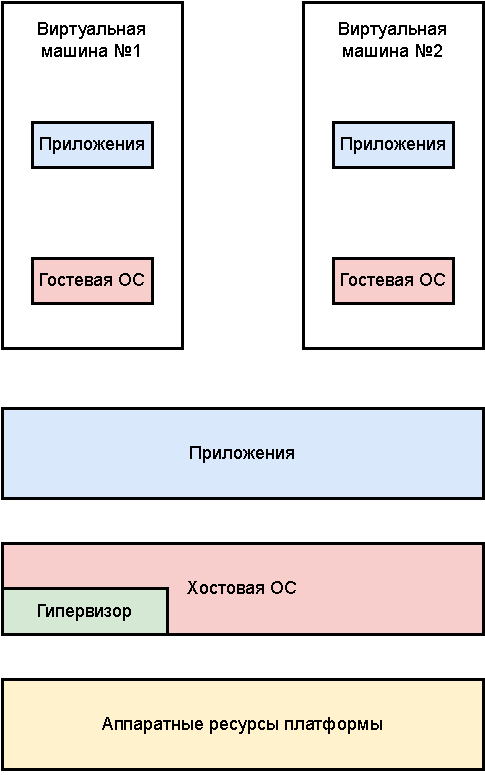
\includegraphics[scale=1]{img/arm-virtualization.pdf}
	\caption{Концептуальная схема системы с поддержкой виртуализации ARM.}
	\label{fig:arm-virtualization}
\end{figure}


\subsubsection{Виртуализация ARM TrustZone}

Технология ARM TrustZone не предназначена для виртуализации, из-за чего в виртуальной среде все виртуальные машины должны использовать одну и ту же доверенную среду исполнения. Такое решение не является эффективным и безопасным: найдя уязвимость в программном обеспечении ДСИ, злоумышленник получает доступ сразу ко всем виртуальным машинам \cite{vtz}.

\subsection{Постановка задачи}

Необходимо разработать и реализовать метод программной реализации ДСИ, который будет удовлетворять следующим условиям:

\begin{itemize}
	\item [---] метод должен работать на процессорах с архитектурой ARMv8 и новее;
	\item [---] необходимо использовать аппаратную виртуализацию ARM;
	\item [---] каждой виртуальной машине должна соответствовать одна независимая доверенная среда исполнения;
	\item [---] метод должен поддерживать все свойства безопасности предоставляемые аппаратной поддерживаемой технология ARM TrustZone (описаны в разделе \ref{arm-trustzone}).
\end{itemize}

\subsection*{Вывод}

В данном разделе представлен обзор следующих реализаций доверенных сред исполнения:

\begin{itemize}
	\item [---] ARM TrustZone;
	\item [---] Intel SGX;
	\item [---] Keystone.
\end{itemize}

Из которых только Keystone является программным решением с открытым исходным кодом, а первые два аппаратными проприетарными решениями.
Сформулированы критерии оценки и проведено сравнение на их основе. Представлен обзор средств виртуализации в процессорных системах ARM. Представлена формализованная постановка задачи на разработку метода программной реализации доверенной среды исполнения с помощью виртуализации процессоров архитектуры ARM.

\pagebreak
